% \renewcommand{\thefigure}{A.\arabic{section}.\arabic{figure}hhh}
\counterwithin{figure}{section}
\setcounter{section}{2} % Assuming section A.2 corresponds to section 2
\setcounter{figure}{0}  % Reset figure counter for this section
\label{Navigation_SupplementaryInformation}


%%%%%%%%%%%%%%%%%%%%
%% SUPPLEMENTARY %%%
%%%%%%%%%%%%%%%%%%%%

\phantomsection
\subsection{Supplementary Plots}


\begin{figure}[ht]
  \centering
  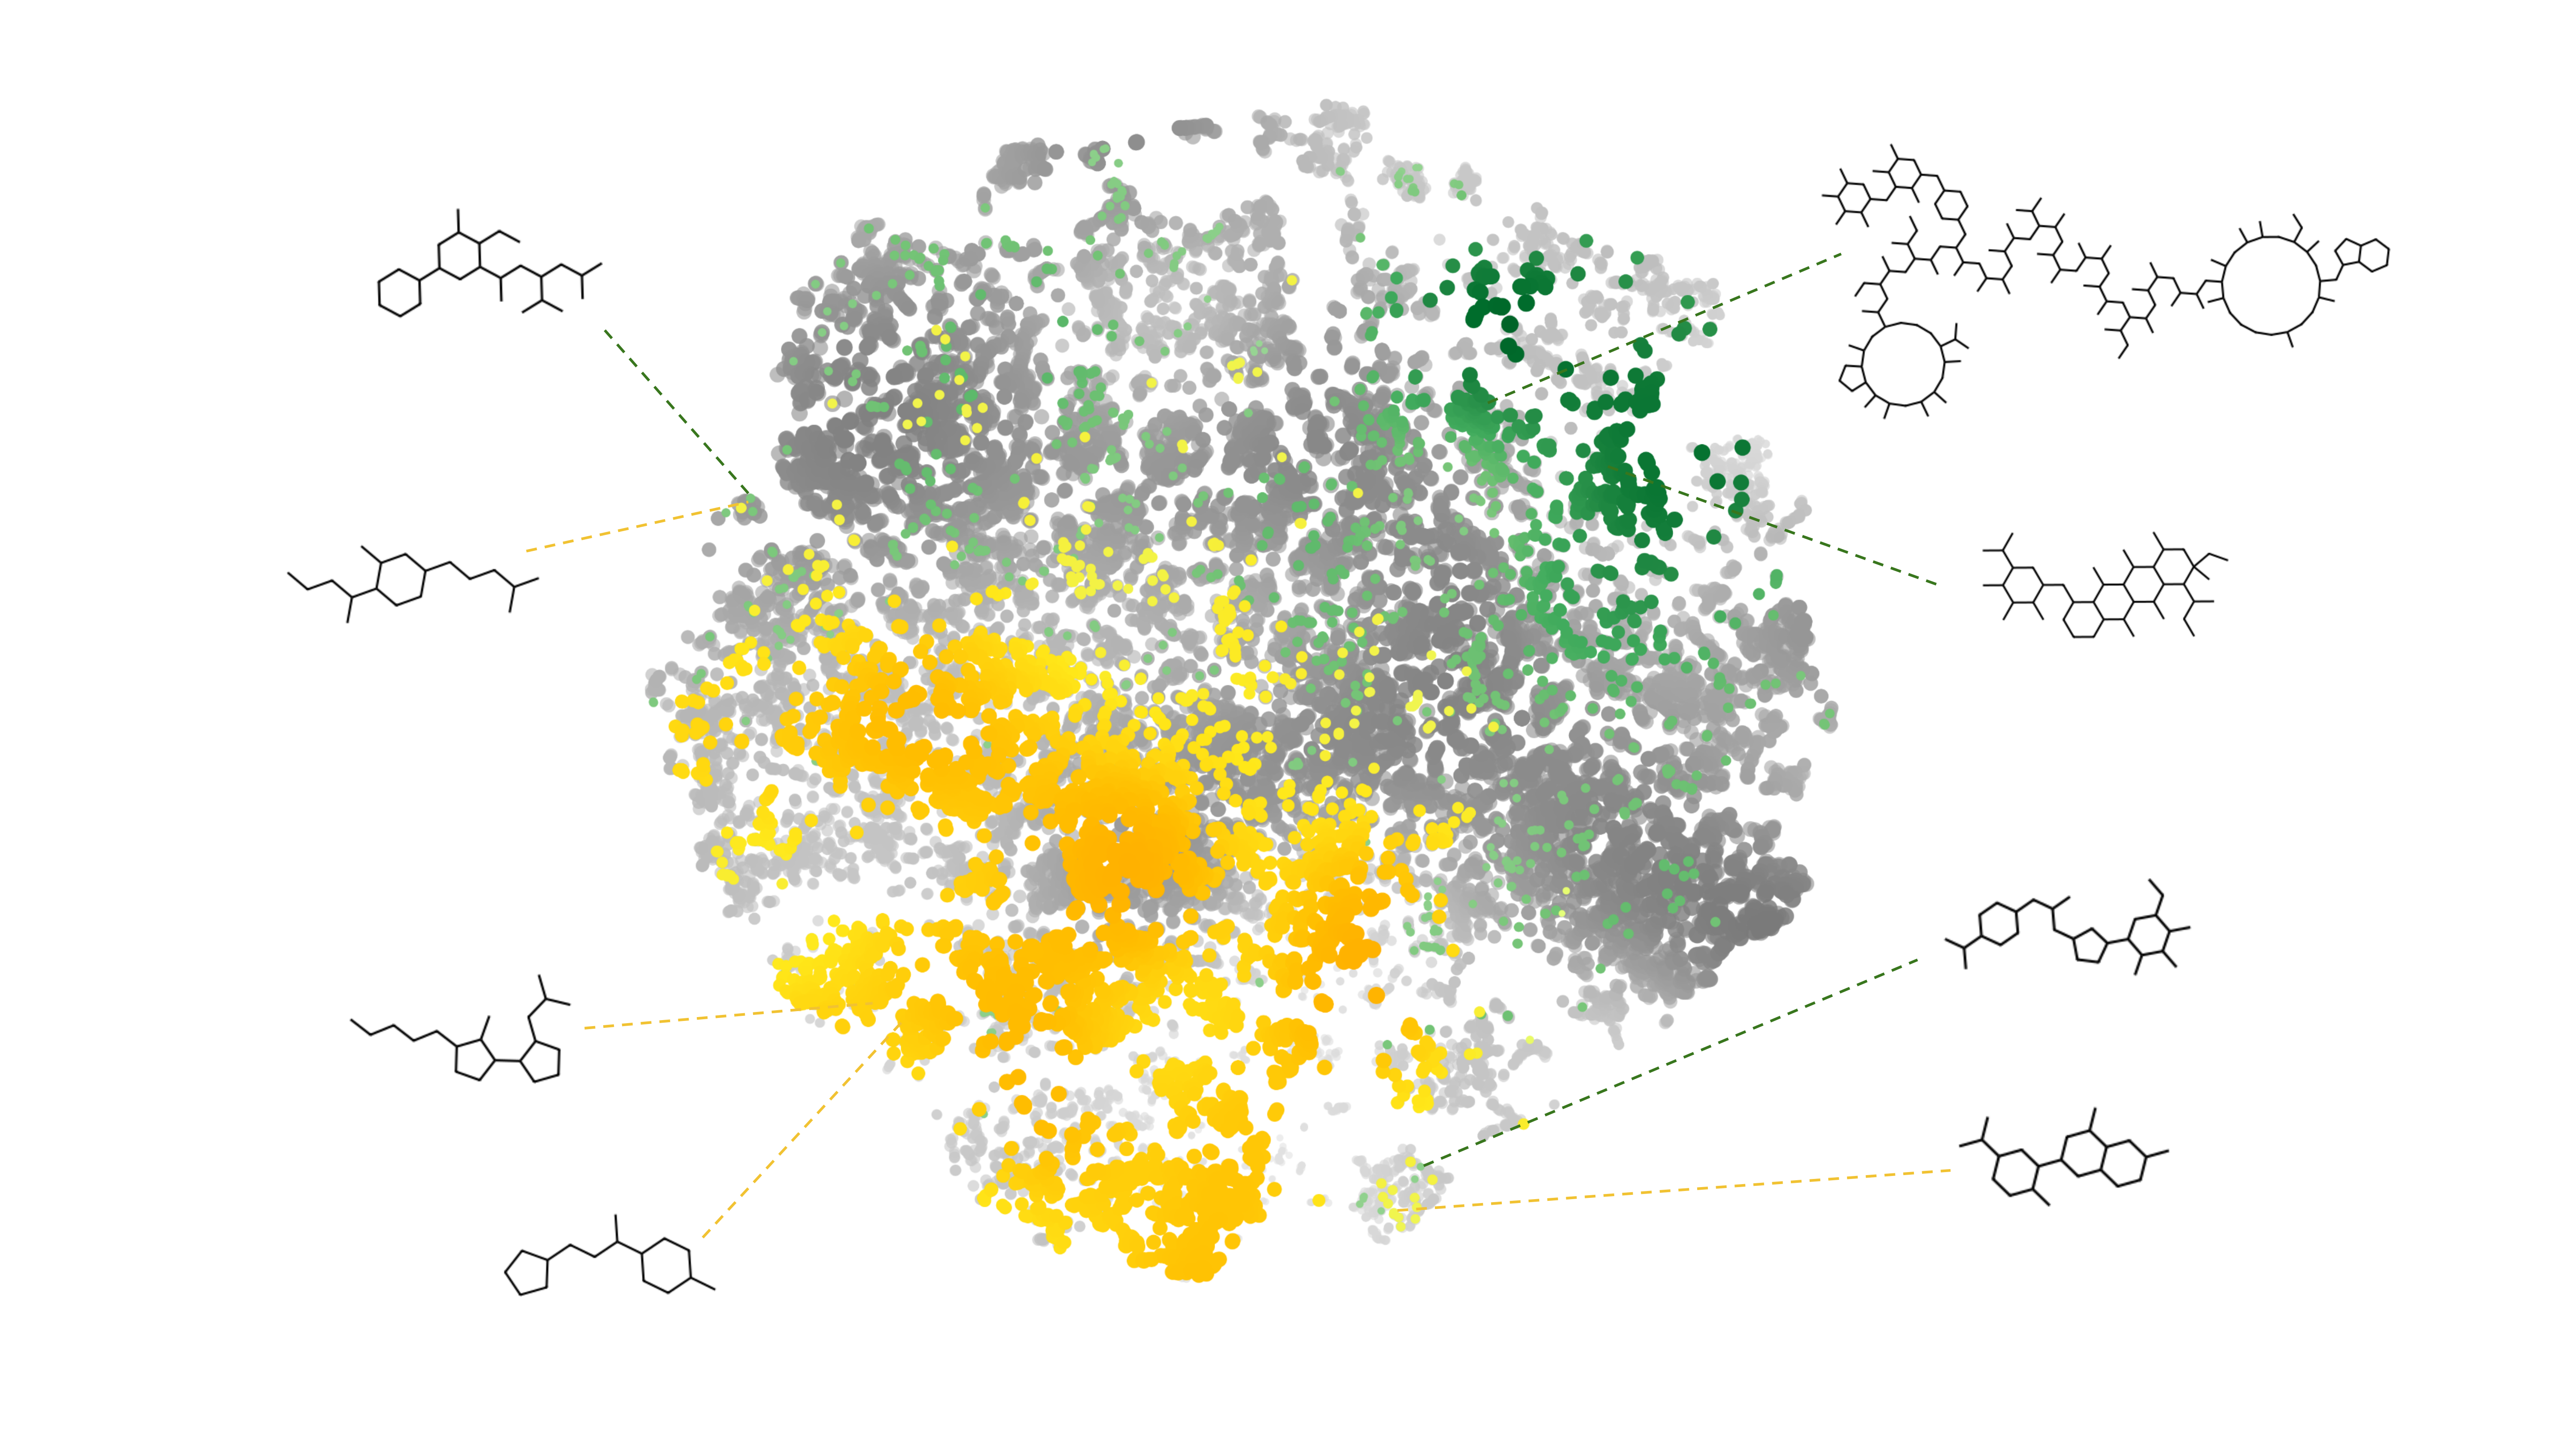
\includegraphics[width=1\linewidth]{figures/Navigation/Supplementary/Medina_v.2.png}
  \caption{2D tSNE representation of the 31,052 selected molecules based on the combined A1-A3-A4 CC signatures (the three spaces are concatenated to obtain 384-length signatures, i.e. 3x128). Green points correspond to Medina’s natural products; yellow points represent 5,000 compounds from the proprietary IRB library. Example molecule scaffolds are displayed for both libraries.
  }
  \label{Navigation_FigS1}
\end{figure}


\begin{figure}[ht]
  \centering
  \includegraphics[width=1\linewidth]{figures/Navigation/Supplementary/filter.png}
  \caption{Physicochemical properties of the 1,521,567 compounds included in the ChemDiv library: presence of PAINS, molecular weight (MW), topological polar surface area (tPSA), alogP, number of hydrogen bond acceptors, number of hydrogen bond donors, number of rotatable bonds, number of aromatic rings and presence in other libraries (the previous version of the IRB Library, the RNA library, the Covalent library and the Fragments library). Green bins indicate compounds that met the established criteria; red bins indicate those that fell outside the criteria.
  }
  \label{Navigation_FigS2}
\end{figure}


\begin{figure}[ht]
  \centering
  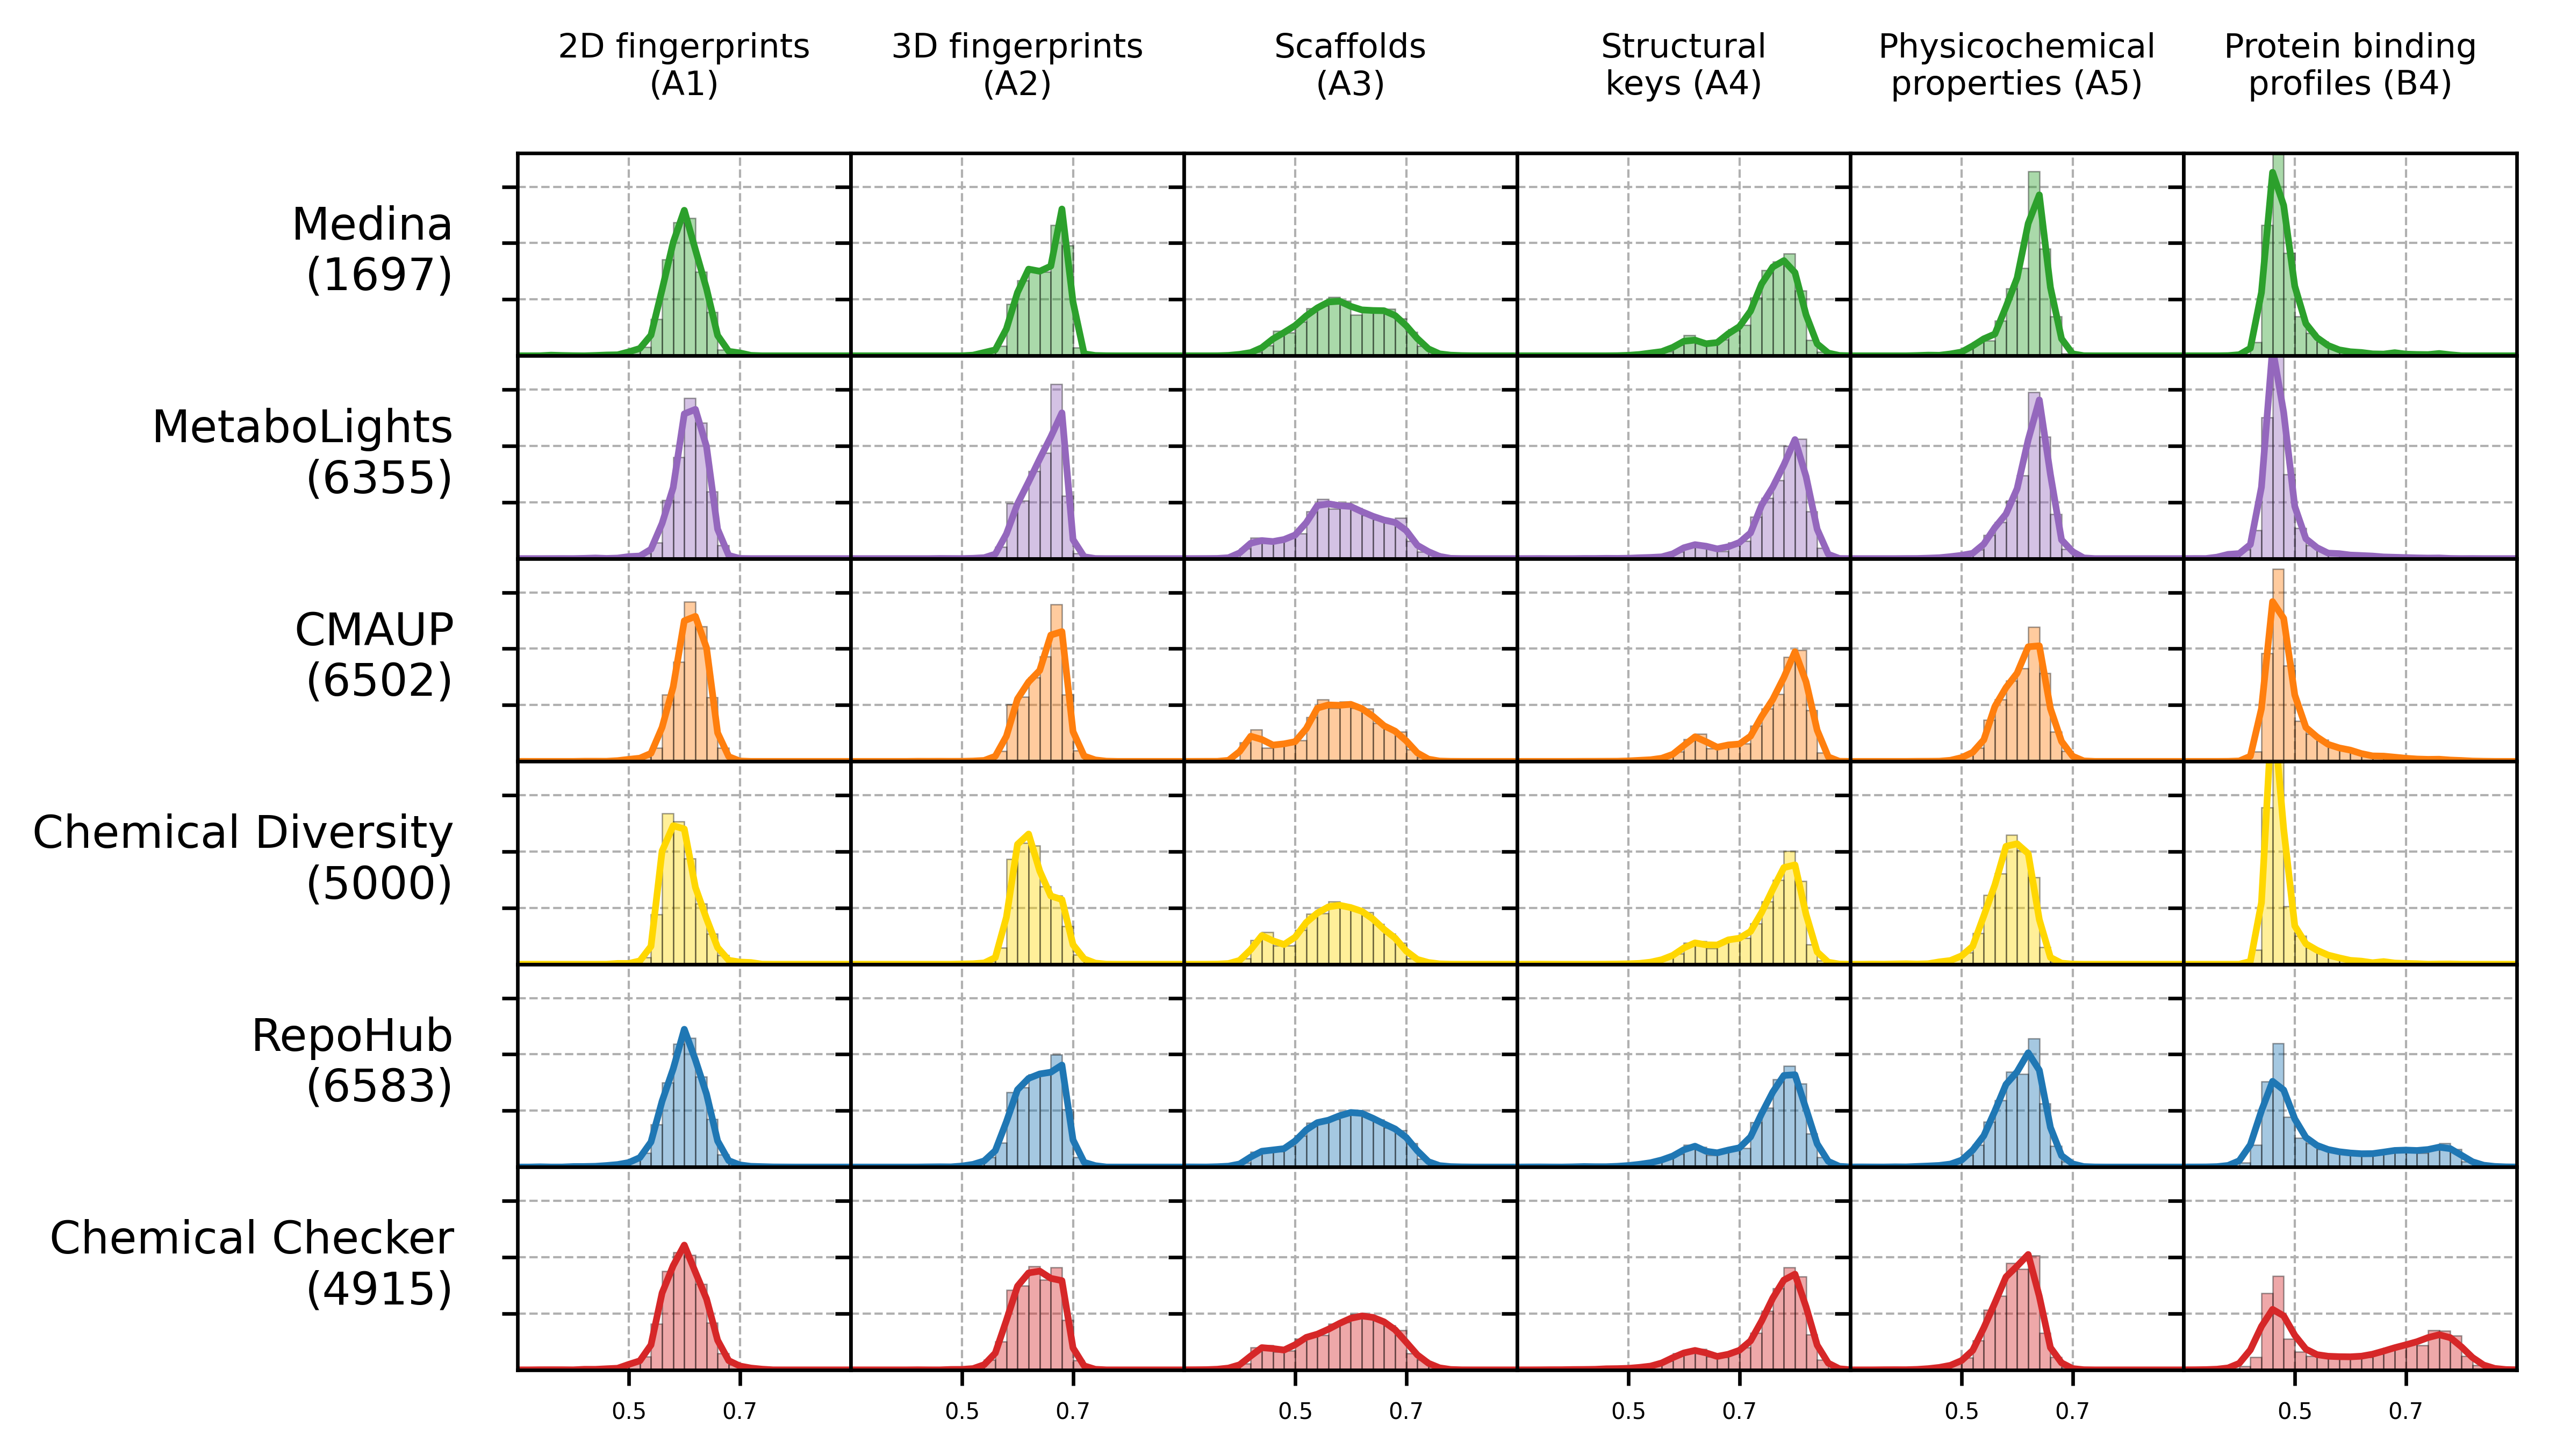
\includegraphics[width=1\linewidth]{figures/Navigation/Supplementary/applicability.png}
  \caption{Distributions of applicability values for the predicted CC signatures (A1-A5 and B4 CC spaces) for the 6 selected compound libraries (Medina, MetaboLights, CMAUP, Chemical Diversity, RepoHub and the Chemical Checker).
  }
  \label{Navigation_FigS3}
\end{figure}

\clearpage
\phantomsection
\subsection{External collaborations}

The external collaborations that contributed to the work presented in \hyperref[Chapter_3.2]{Chapter 3.2} are listed as follows:

\begin{enumerate} 
\item[\textbullet] Collaboration with the IRB Drug Screening Platform aimed at designing a new version of the IRB proprietary library from multiple sources, including chemically diverse compounds, covalent inhibitors, fragments, etc. 
\item[\textbullet] Collaboration with Fundacion MEDINA, a non-profit research organization, based in Granada, Spain, and focused on the discovery of new drugs from natural products. The collaboration was centered on compound library signaturization and visualization, involving the MEDINA collection of natural products.
\end{enumerate}

Apart from the ones mentioned above, the course of the PhD also led to numerous external collaborations related with chemical and bioactivity signatures, not included in \hyperref[Chapter_3.2]{Chapter 3.2} for the sake of clarity and focus. 

